% MUST use a4paper option
% MAY use twoside, smaller font, and other class - but not for Självständigt arbete i IT
\documentclass[a4paper,12pt]{article}
% Use UTF-8 encoding in input files
\usepackage[utf8]{inputenc}
% Use T1 font encoding to make the \hyphenation command work with UTF-8
\usepackage[T1]{fontenc}

% Om ni skriver på svenska, använd denna rad:
% \usepackage[english,swedish]{babel}
% If you are writing in English, use the following line INSTEAD of the previous (note order of parameters):
\usepackage[swedish,english]{babel}

% Use the template for thesis reports
\usepackage{UppsalaExjobb}

\usepackage{enumitem}
\usepackage{svg}
\usepackage{subcaption}
\usepackage{caption}
\usepackage{mwe}

% För att göra ett index behövs
%  - \usepackage{makeidx}
%  - \makeindex i "preamble", dvs före \begin{document}
%  - \printindex, typiskt sist, före \end{document}
% - och att man lägger in \index{ord} på olika ställen i dokumentet
\usepackage{makeidx}
\makeindex


% Designval: per default används styckesindrag, men ibland blir det snyggare/mer lättläst med tomrad mellan stycken. Det åstadkoms av de följande raderna.
% Tycker ni om styckesindrag mera, kommentera bort nästa två rader.
\parskip=0.8em
\parindent=0mm

% Designval: vill ni ha en box runt figurer istället för strecken som är default, av-kommentera raden nedan. Obs att både \floatstyle och \restylefloat behövs.
%\floatstyle{boxed} \restylefloat{figure}

\begin{document}
% För att ställa in parametrar till IEEEtranS/IEEEtranSA behöver detta ligga här (före första \cite).
% Se se IEEEtran/bibtex/IEEEtran_bst_HOWTO.pdf, avsnitt VII, eller sista biten av IEEEtran/bibtex/IEEEexample.bib.
%%%% OBS: här ställer ni t.ex. in hur URLer ska beskrivas.
\bstctlcite{rapport:BSTcontrol}

% Set title, and subtitle if you have one
\title{Allocators in OpenJDK} % och uppsatsmetodik
% Use this if you have a subtitle
%\subtitle{beskrivande men gärna lockande}
%\subtitlesubtitle

% Set author names, separated by "\\ " (don't forget the space, or use newline)
% List authors alphabetically by LAST NAME (unless someone did significantly more/less, which should not be the case)
% For drafts, include your email addresses to make it easier to send peer reviews
\author{Casper Norrbin}

% Visa datum på svenska på förstasidan, även om ni skriver på engelska!
\date{\begin{otherlanguage}{swedish}  %\foreignlanguage doesn't seem to affect \today?
    Juni 2024
  \end{otherlanguage}}

% Använd detta om året för rapporten inte är innevarande år
%\year=2018

% Ange handledare, ämnesgranskare, examinator om dessa finns
\handledare{Erik Österlund}
% There is also \exthandledare
\reviewer{Tobias Wrigstad}
\examinator{Lars-Åke Nordén}

% This creates the title page
\maketitle

% Change to frontmatter style (e.g. roman page numbers)
\frontmatter

%%%% OBS: Läs också källkoden till alla text/X.tex.
%%%% Tips: ni kan använda separata filer för de olika delarna i er rapport på motsvarande sätt,
%%%% men använd inte samma filnamn!

\begin{abstract}
  
%%% Local Variables:
%%% mode: latex
%%% TeX-master: "main"
%%% End:
Memory fragmentation is a common issue in programs running with dynamic memory allocations. Java is a programming language that solves the problem of memory fragmentation by using garbage collectors. The most recent garbage collector added to Java, ZGC, solves fragmentation by moving objects around in memory, leading to more densely packed allocations. ZGC performs sequential allocations with the use of a bump-pointer, which offers great execution times, but has the issue of causing fragmentation due to its inability to reach certain areas of free memory.

This thesis present a new solution to compacting memory in ZGC using free-list based allocators. By using free-lists to represent the fragmented memory as available space, allocations can utilize the previously considered unreachable memory as a target location for compaction. The trade-off of introducing this new allocation strategy is a more computationally heavy allocation method, but more total memory that can be utilized for compaction. Results from this thesis show promising results when utilizing an optimized version of a TLSF allocator, showing good possibilities of moving objects into fragmented memory.


% in programs that run for longer periods of time. By continuously alternating between allocating and releasing memory, the program can cause the memory to become fragmented, meaning objects are no longer stored in a contiguous block of memory. The free regions of memory between objects can then be hard to utilize, because certain objects might not fit in that space. In programming language with dynamic memory management, this issue can be solved by a garbage collector which automatically frees up memory that is no longer in use. Different garbage collectors have different strategies for managing memory, but they all aim to reduce fragmentation and improve the performance of the program. In this thesis, we will explore the use of free-list allocators in garbage collectors, and its integration in one of Java's latest garbage collectors, ZGC. ZGC uses bump pointers to allocate memory which allows for fast allocations. However, it is known that bump pointers can cause fragmentation in the memory. The goal of using a free-list allocator is to let the garbage collector know that there is free space available in between allocations, which is something that bump pointers are not able to do. We will investigate the feasibility of using such an allocator and how it can be used to compact memory.


\end{abstract}

\begin{sammanfattning}
  \input{text/sammanfattning}
\end{sammanfattning}

% Innehållsförteckningen här.
\tableofcontents

% Här kan man också ha \listoffigures, \listoftables

\cleardoublepage

% Change to main matter style (arabic page numbers, reset page numbers)
\mainmatter

% Here comes the text of the report.

\section{Introduction}
\label{sec:introduction}

%%% Local Variables:
%%% mode: latex
%%% TeX-master: "main"
%%% End:
%The goal of this thesis project is to investigate the possibility of using free-list allocators in garbage collectors. The project will focus on integrating a free-list allocator in the ZGC, a garbage collector available in the most recent release of the OpenJDK. Currently in ZGC, memory is allocated in regions using sequential allocators, discussed in more detail in Section~\ref{sec:background}. Although it is a very performance effective way of allocating objects, it is known that bump pointers can cause a lot of external fragmentation in the memory~\cite{TODO:bump}. By making use of a free-list allocator, it is possible to let the garbage collector know that there is free space available in between allocations, allowing for allocations inside of the externally fragmented memory. This will add some extra work load on the allocation of objects, but will allow for using memory more efficiently. The project will investigate the feasibility of using such an allocator, and whether it improves the throughput and or memory usage.
Garbage collection is a feature in many programming languages with dynamic memory allocations, where the task of a garbage collector is to keep track of which parts in the memory is currently being used by the running program. This makes it possible for the garbage collector to automatically free up unused memory allocations. Efficient memory management is useful for increasing the performance and resource usage of programs, since all of the memory utilization is heavily relying on how the memory is being kept track of by the underlying garbage collector.

Java is a programming language with dynamic memory management that makes use of garbage collectors in order to handle memory. Java is used by one of the largest services on Earth, Netflix. Operating within a runtime environment known as the Java Virtual Machine (JVM), Java allows users to configure the JVM for optimal performance, including the choice of garbage collector. In Mars 2024, a blogpost from Netflix was released~\cite{netflix:zgc}, announcing the benefits of switching from one garbage collector, to the latest, most modern garbage collector, generational ZGC. They found that the upgrade yielded an improvement of 6-8\% percent in CPU utilization, proving that new technologies can lead to great improvements.

This thesis will continue on the subject of further exploring possible improvements that can be made to the JVM and its garbage collectors. Specifically, the goal is to look at the possibility of implementing a new method for allocating objects inside fragmented memory where previously allocated objects have been found to be unreachable. In ZGC, this is not an available feature, since it opts for using bump pointers instead. In Section~\ref{sec:memory_allocation}, the difference between bump pointers and free-list based allocations is explained in more detail. With a new allocator in place which can handle allocations in free-lists, a new method for compacting memory would be available where objects can be allocated in non-contiguous regions of free memory, which is what this thesis will investigate the feasibility of doing.

The integration of a new allocation method meant that changes had to be done to how ZGC handles 

\subsection{Purpose and Goals}
\label{sec:purpose}

The goal of this project is to investigate to what extent a free-list-based allocator can be used to reduce intra-page fragmentation in a garbage collector. Most garbage collectors utilize bump-pointer allocation, enabling swift allocation and deallocation. However, the utilization of a bump-pointer allocator introduces certain drawbacks. One notable limitation is that a free-list-based allocator possesses the flexibility to allocate objects anywhere within a page, as opposed to being confined to the specific location indicated by the top-pointer in a bump-pointer approach. This inherent inflexibility in bump-pointer allocation may contribute to increased intra-page fragmentation, as objects are allocated strictly at the top of the available memory, potentially leaving unused space within the page.

We will explore what adaptions can be made to adapt an existing free-list-based allocator to be used in ZGC, a garbage collector in the OpenJDK, in addition to specific use-cases that could benefit from using the allocator as opposed to bump-pointer allocation.

%%% Local Variables:
%%% mode: latex
%%% TeX-master: "main"
%%% End:


\subsection{Delimitations}
\label{sec:delimitations}

The main limitation of this project is that we will not be integrating the allocator into ZGC and OpenJDK. A scope of 20 weeks is deemed not enough to implement, adapt, evaluate and also integrate an allocator. Integration will be considered as future work.

% Linux?
% Small pages?

%%% Local Variables:
%%% mode: latex
%%% TeX-master: "main"
%%% End:


\subsection{Individual Contributions}
\label{sec:individual_contrubitons}

This thesis was written primarily by Niclas Gärds, but Section 2 was coauthored by Joel Sikström and Casper Norrbin. More specifically, section 2.1, 2.2, 2.3 was written by Joel, and 2.4 was written by Casper Norrbin.


%%% Local Variables:
%%% mode: latex
%%% TeX-master: "main"
%%% End:


\paragraph{Acknowledgement}
I would like to thank my supervisor Erik Österlund and subject reviewer Tobias Wrigstad for their fantastic help throughout this thesis project. Their expertise in the subject offered great guidance during the entirety of the project. I would also like to thank the people at Oracle for providing a great workplace environment, where I felt welcome to ask for help at any time.

%%% Local Variables:
%%% mode: latex
%%% TeX-master: "main"
%%% End:


\newpage
\section{Background}
\label{sec:backgrond}
\input{text/background}

\subsection{Memory Management}
\label{sec:memory_management}

Memory management is typically categorized into being either manual or automatic. Manual memory management involves explicitly assigning and managing memory by the programmer, which is commonly used in low-level languages like C and C++. Automatic memory management is handled automatically by the system, without the need for the programmer to intervene. One method for achieving automatic memory management is through the use of a garbage collector, a mechanism responsible for both allocating and releasing memory. Languages like Python and Java are examples of programming languages that do this.

Memory is most commonly allocated during runtime of the program as opposed to allocating everything in advance, during startup for example. The process of allocating memory during runtime is referred to as dynamic memory management, which presents a number of challenges for reliably being able to satisfy allocation requests and run for extended periods of time.

The main problem with dynamic memory allocation is that an allocation might fail due to memory exhaustion. Exhaustion may arise either due to the program requiring more memory than is available in the system or from the circumstance where free memory is available but cannot be reused. The second case is sometimes referred to as just wasted memory, but to be precise we will classify it as either internal or external fragmentation, which will be discussed further below.

%%% Local Variables:
%%% mode: latex
%%% TeX-master: "main"
%%% End:


\subsection{Fragmentation}
\label{sec:fragmentation}

As mentioned above, we classify fragmentation as being either internal or external. Internal fragmentation is considered wasted space due to alignment and it may sometimes be required for an allocator to allocate a slightly smaller block of memory than a user has requested. Figure~\ref{fig:internal_fragmentation} shows an example of when a user has requested 100 bytes, which has required the allocator to allocate 128 bytes instead due to alignment, where the last 28 bytes as wasted space.


\begin{figure}[H]
    \centering
    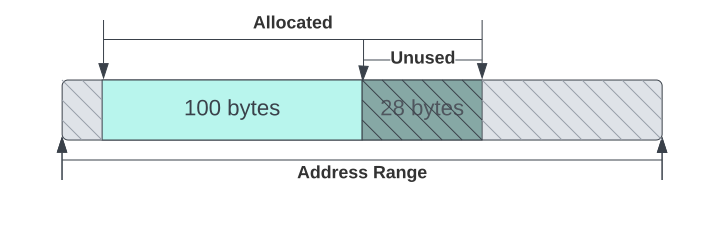
\includegraphics[width=0.75\textwidth]{figures/internal_fragmentation.png}
    \caption{A memory region containing one allocated piece of memory that is 128 bytes large. However, the user only requires 100 bytes of those and thus, 28 bytes is wasted.}
    \label{fig:internal_fragmentation}
\end{figure}

External fragmentation occurs when there is enough memory available in total but dispersed in smaller, non-contiguous chunks. This is illustrated in Figure~\ref{fig:external_fragmentation}, where a total of 80 bytes is available in total, distributed in the memory region. However, the user is unable to allocate more than 32 bytes due to the smallest uninterrupted memory chunk being only this size.

\begin{figure}[H]
    \centering
    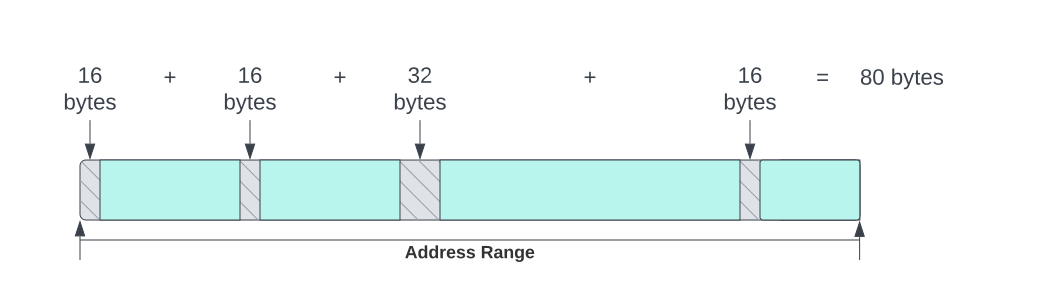
\includegraphics[width=0.8\textwidth]{figures/external_fragmentation.png}
    \caption{A memory region containing several allocated blocks with unused space in between them. Although the total sum of the unused portions is large, a request of more than 32 bytes cannot be fulfilled.}
    \label{fig:external_fragmentation}
\end{figure}

% Beskriva skillnad mellan internal och external fragmentation och att de kan anses som samma sak, "wasted space" (TLSF paper).

% Kanske fixa två figurer som visar på exakt vad det handlar om (om det är relevant)?

%%% Local Variables:
%%% mode: latex
%%% TeX-master: "main"
%%% End:


\subsection{Memory Allocation}
\label{sec:memory_allocation}

In this section we will describe two fundamental allocation strategies, called sequential allocation and free-list allocation, in addition to the more complex case of using multiple free-lists.

\subsubsection{Sequential Allocation}
% Describe bump-pointer/sequential/linear allocation.

Sequential allocation represents one of the most straightforward methods for allocating memory within a contiguous chunk of memory. In this approach, a pointer is used to keep track of the current position within the memory chunk. As new objects are allocated, the pointer is moved forward by the size of the object and any necessary padding or alignment. Sequential allocation is also known as 'bump-pointer allocation' due to the incremental 'bumping' of the pointer with each new allocation. It is a simple and efficient method, particularly suitable for scenarios where memory is managed linearly. Despite its simplicity, sequential allocation can be highly effective in situations where memory fragmentation is not a significant concern and where a predictable, sequential layout is desirable.

While this approach is easy to implement, it may not be the most suitable choice for all scenarios, especially in systems with varying memory demands or those requiring more sophisticated memory management strategies. Nevertheless, its simplicity makes sequential allocation a valuable technique in specific use cases.

\subsubsection{Free-List Allocation}
An alternative to sequential allocation is free-list allocation, which records the location and size of free blocks in a data structure, such as a linked list for example. In the simplest form one would use a single list for storing free blocks. An allocator would then consider each block in a sequential manner and choose one according to some policy. Below we will give an overview of how the most common policies work.

\begin{description}
    \item[First-fit]
        The first block that is large enough for satisfying a request will be used. This minimizes search time, but does not consider that there might exist a more suitable block elsewhere in the free-list. This search is restarted from the list's head for each new request. 
    \item[Next-fit]
        Searching for a block is initially done in the free-list like what is described for first-fit. In subsequent searches however, it resumes from where the previous search concluded, enhancing efficiency when searching for a new block. This approach is based on the observation that small blocks often accumulate at the start of the free-list, streamlining the search space by starting further into the list in the next iteration.
    \item[Best-fit]
        The entire free-list will be searched until the smallest available block that can satisfy a request is found. The main benefit of best-fit is that fragmentation is minimized at the cost of additional search time.
\end{description}

The three policies described above, and many others, have in common that when a block that is larger than what is requested is found, it is split up. We generally want to split block as infrequently as possible to have larger blocks available for larger request sizes. If blocks are split too often, many small blocks might accumulate, which might increase external fragmentation to a level where new requests cannot be fulfilled. Additionally, splitting blocks less frequently will also mean less merging, or coalescing, of blocks to larger sizes, which could improve performance.

\subsubsection{Segregated-Fit Allocation}
Instead of using a single free-list where blocks of many sizes are stored, one might instead use multiple free-lists that store blocks of similar sizes or size ranges, called segregated-fit. The ambition of using multiple free-lists is to narrow down the search space to fewer blocks, allowing us to find blocks large enough to satisfy a request faster. However, there is an added overhead of storing a pointer to the head of each free-list which is usually insignificant. It is crucial to note that blocks are logically segregated into their respective free-lists based on size but are not required to be physically adjacent in memory within the same free-list. This distinction emphasizes the organizational structure of segregated-fit.

Segregated-fit is often employed in real-time systems where predictable and efficient memory allocation is crucial. The reduced search space and minimized search time to find suitable blocks allows timing constraints to be met.

%%% Local Variables:
%%% mode: latex
%%% TeX-master: "main"
%%% End:


\newpage
\subsection{Garbage Collection}
\label{sec:gc}
As previously mentioned, garbage collection is a method of achieving automatic memory management where the system identifies and cleans up unused objects, which are considered garbage. This removes the requirement of managing memory from the user, which reduces the possibility of memory related issues occurring. This also removes some control from the user, and could lead to sub-optimal usage of system memory.

%%% Local Variables:
%%% mode: latex
%%% TeX-master: "main"
%%% End:


\subsection{OpenJDK}
\label{sec:openjdk}

OpenJDK~\cite{openjdk} is a set of tools for creating and running Java programs, maintained by Oracle. HotSpot~\cite{hotspot} is one of these tools and the reference implementation of the Java Virtual Machine (JVM)~\cite{JVM}. Specifically, a virtual machine (VM) emulates a distinct computer in order to run various programs, which could be anything from full operating systems - to more specialized machines. Hence, the JVM is designed specifically to execute Java programs. It translates programs to instructions for the underlying machine, creating an abstraction of the hardware of the physical machine and allows Java programs to be run on any platform that the JVM runs on.

HotSpot is compromised of several components for running Java applications, such as an interpreter, a Just-In-Time (JIT) compiler, and a garbage collector (GC). In combination, these components provide the means for running different types of Java programs on the platforms supported by HotSpot.

%%% Local Variables:
%%% mode: latex
%%% TeX-master: "main"
%%% End:



\subsection{The Z Garbage Collector}
\label{sec:zgc}

ZGC is a garbage collector available in the OpenJDK. It was introduced as an experimental implementation in OpenJDK 11, but was declared production ready in OpenJDK 15. ZGC is modern, generational, region-based, parallel garbage collector that aims to keep pauses at a constant time even though the heap size increases. This means latency will remain low as the heap size increases.%~\cite{zgc:deepdive}.

%%% Local Variables:
%%% mode: latex
%%% TeX-master: "main"
%%% End:


\subsubsection{Pages}
\label{sec:zpage}
When using the ZGC, memory is stored in regions, which is referred to as pages. Pages are classed as \textit{Small}, \textit{Medium} or \textit{Large}. When new objects are allocated, they are allocated inside of these pages. An illustration of how the allocation of new objects in pages, as well as garbage collection inside of the page is shown in Figure~\ref{fig:zpages}.

%bild1 tom page
%bild2 page med 2 allokeringar
%bild3 pafge med en av allokeringarna markerad som LIVE och en DEAD
%bild4 page som visar att de är external fragmentation
\begin{figure*}
    \centering
    \begin{subfigure}[b]{0.475\textwidth}
        \centering
        \includesvg[scale=0.4]{figures/zpage_empty}
        \caption[Network2]%
        {This image shows the state of a newly allocated Z-Page where no objects have yet to be allocated inside it.}    
        \label{fig:page:empty}
    \end{subfigure}
    \hfill
    \begin{subfigure}[b]{0.475\textwidth}  
        \centering 
        \includesvg[scale=0.4]{figures/zpage_allocated}
        \caption[]%
        {This image shows a scenario where two objects of size 64B and 128B respectively have been allocated to the empty Z-Page.}    
        \label{fig:page:allocated}
    \end{subfigure}
    \vskip\baselineskip
    \begin{subfigure}[b]{0.475\textwidth}   
        \centering 
        \includesvg[scale=0.4]{figures/zpage_liveness}
        \caption[]%
        {This image represents the aftermath of doing a liveness check after the pointer to the first object has been lost. This means that the first object is considered dead, but the second object is still alive.}    
        \label{fig:page:liveness}
    \end{subfigure}
    \hfill
    \begin{subfigure}[b]{0.475\textwidth}   
        \centering 
        \includesvg[scale=0.4]{figures/zpage_fragmented}
        \caption[]%
        {After the garbage collection cycle, if the page was not relocated due to other pages being prioritized the page ends up with externally fragmented memory. The 64B at the top of the page will not be usable.}    
        \label{fig:page:fragmented}
    \end{subfigure}
    \caption[]
    {A representation of the allocated memory inside of a Z-Page} 
    \label{fig:zpages}
\end{figure*}
As can be seen in Figure~\ref{fig:page:fragmented}, there is going to some external fragmentation because of how the pages make use of the bump pointer in order to allocate new objects, effectively meaning the freed object at the top is still allocated because the program is no longer able to allocate new objects in its place. To counter this, and make the memory usable again, the ZGC uses relocation. Relocation is done by moving all of the live objects from one page to other pages. Three different things might happen here:\\
\begin{enumerate}
    \item There are pages with usable memory: This means that the objects that are going to be relocated can be placed in pre-existing pages, and the evacuated page can be freed entirely. 
    \item All pages are full: When all pages are full, the objects cannot simply be moved to other existing pages, but instead have to allocate an entirely new page. This new page is where the objects are going to be evacuated to. This removes fragmentation because the new page will have stored all of the objects in a continuous manner.
    \item The heap is full: When there are no pages with free memory, and there is no room to allocate new pages, the only way to free up space is by performing an in-place compaction. This effectively means the objects are being replaced inside of the current page that they are in. This will compact the page and remove any external fragmentation, at the cost of being a very expensive operation.
\end{enumerate}

In Figure~\ref{fig:relocation_scenarios} all three scenarios are illustrated by examples of what the heap may look like with some amount of pages with objects allocated inside them.

\begin{figure}
    \centering
    \includesvg[scale=0.5]{figures/zpages_relocation}
    \caption{Illustration of the three scenarios of relocation.}
    \label{fig:relocation_scenarios}
\end{figure}
%%% Local Variables:
%%% mode: latex
%%% TeX-master: "main"
%%% End:


\section{Related work}

%%% Local Variables:
%%% mode: latex
%%% TeX-master: "main"
%%% End:

In this section, we review research that has already been done on this subject. By looking at what has been done previously, the goal is to build up knowledge about what more there is to explore, and how this thesis project will build upon what they have discovered. 

\subsection{ZGC}
As ZGC is the main topic of this thesis, and is the reason this thesis exists, it is only fitting to cover some of the previous research that has been done in order to improve ZGC. The first paper is one from 2019 about \textit{Improving relocation performance in ZGC by identifying the size of small objects}, written by Jinyu Yu~\cite{TODO:https://www.diva-portal.org/smash/get/diva2:1693010/FULLTEXT01.pdf}. This paper researched the option of reducing the amount of relocations being done for compaction by introducing a new classification for object sizes in ZGC. The results from this paper show that it is a valuable effort to try reducing the amount of relocations being done. With a decrease of about 40\% of all relocations, the throughput stayed unchanged during most benchmarks used for evaluation. This thesis will also explore a new way of relocating objects, but define a new way of representing the relocation destination.

Another paper was written by L. Shoravi, where he explored the option of compressing pointers in ZGC~\cite{TODO:https://www.diva-portal.org/smash/get/diva2:1766097/FULLTEXT01.pdf}. The mission of copmressing pointers is to reduce the amount of memory used by the garbage collector. While this thesis does not use compression for reducing the amount of memory used by the garbage collector, the goals is to use memory more efficiently, and reduce fragmentation, which is also a way of reducing the overall memory usage of the garbage collector.

C. Tauro et. al. wrote a paper on the comparison of two different garbage collectors in Java, CMS and G1~\cite{https://citeseerx.ist.psu.edu/document?repid=rep1&type=pdf&doi=6b97a988da6f82e13ea5fc673c72b463a30b98db}. CMS, in contrast to the garbage collector studied in this thesis, ZGC, uses free-lists to represent available memory in the heap. In the paper, they find that CMS performs significantly better in memory usage than what is observed by looking at G1, another regional garbage collector. However G1 performance marginally better when it comes to throughput, according to their evaluations. This suggests that they both have benefits that can be desirable when running certain program. This is further motivates the work of this thesis, which is to combine the regional characterstic of ZGC and G1, and the usage of a free-list based allocator like in CMS, and look at the possibility of finding desirable outcomes when they both work together.

\section{Theory}
\label{sec:theory}

%%% Local Variables:
%%% mode: latex
%%% TeX-master: "main"
%%% End:

This section continues on the topic of different allocation methods presented in Section~\ref{sec:background}. Depending on which allocation method is chosen, the system in use will be more equipped for certain tasks than others. Different scenarios where one allocator would be more suitable than the other is going to be explained in this section.

\subsection{Using Bump Pointers}
For a further explanation of bump pointers, see Section~\ref{sec:memory_allocation}.

Bump pointers are commonly used in systems where the allocation of objects should happen very fast, as the allocation can be done in constant time. It is also very well suited for parallel programs, since the act of moving the bump pointer to its next location when doing an allocation can be done atomically. 

But bump pointers are bad at XXXXXXX.

\subsection{Using Free Lists}
Free list is good at XXXXXXXXXX

But bad at XXXXXXXXXXXX

\subsection{Combining Both}
In certain scenarios it might be beneficial to use both free lists and bump pointers. This is because the free list allocator is able to handle allocations in a more efficient way, while the bump pointer allocator is more suitable for parallel programs. TODO continue on the topic of trying to switch between the two allocators.

\section{Method}
\label{sec:method}

%%% Local Variables:
%%% mode: latex
%%% TeX-master: "main"
%%% End:

\subsection{Integration Method}
% https://ieeexplore.ieee.org/stamp/stamp.jsp?tp=&arnumber=6312870 källa kanske. 1975 LOL

This thesis employs a cyclical development method for integrating a new feature into an existing codebase. The approach is designed to iteratively refine the integration through repeated iterations of evaluation and modification.

\begin{description}
  \item[Phase 1: Analysis]
  The initial phase involves a detailed examination of the system to identify areas impacted by the integration of the new feature. This involves an in-depth review of the existing code, experimental adjustments to observe possible impacts, and consultations with the code's original developers. The purpose of this phase is to gain a comprehensive understanding of the system's functionality and dependencies, which facilitates accurate identification of critical modification points.
  
  \item[Phase 2: Iterative Integration]
  Following the preliminary analysis, the integration ph-ase proceeds in an iterative manner. It begins with creating an implementation design, derived from the insights gained during the analysis phase. The integration then proceeds with applying the planned changes, followed by testing to evaluate the correctness and impact of these changes. If the integration achieves the expected outcomes, the process is completed. If not, the feedback from testing informs further refinements in the plan, and the cycle repeats - designing, implementing, and testing — until the integration fully aligns with the desired functionality, and programs are executed without errors.
\end{description}

This cyclical method offers a systematic approach to implementing new functions in a large code base. By iteratively improving the design, and always making sure to assess the current iterations impacts on the code before moving on to further changes, the final implementation is less prone to fail.

% This project outlines the integration of a new feature in a large code base. New implementations in large code bases tend to have bigger impacts than intended since it is hard to know which parts of the system are going to be impacted. The integration method used during this thesis consists of two different phases, the identification phase, and then the implementation phase. 

% The goal of the first identification phase is to study the behavior of the program in the areas that are going to be impacted. This involves reading the code, changing the code to see the impacts, and also talking to the authors of the code to better understand what implications a small change might have. The goal is that by the end of this phase, enough information will be gathered about the different parts of the system such that it would be easier to identify which parts of the code have to be changed to implement the new feature.

% The second phase involves the process of actually implementing the desired changes. Firstly, a design of the implementation is made from the gathered knowledge of the identification phase. Following this, an iterative method of implementing the design and testing it is done. If the implementation works as intended, the implementation is considered done, and if the implementation does not work as intended, the implementation phase is restarted and a new design has to be made from the knowledge gathered from the failed tests.

\subsection{Exploratory Programming}
The main method for implementing new changes to the JVM code was using exploratory programming. This method implies making changes to the code and seeing what impacts the changes have based on data that is collected from the program. Some tools used to facilitate this process were debuggers and logging tools. In this section, I explain two useful tools that simplify the process of understanding the code.

\subsubsection{Debuggers}
A debugger is a tool that can run your program with an interface to let the developer know the values of certain variables or locations of memory addresses. A useful tool used during this project is the \textit{rr\_debugger}, designed by O'Callahan et al.~\cite{rrdebugger}, which can be used to record and replay a program's execution with deterministic behavior. This makes it possible to view parts of the program at different times. This is very useful in the context of the OpenJDK since the code consists of several hundreds of thousands of lines of code, which makes it easy to have different parts of the system interacting with each other without the developer knowing. Finding which areas in the code are causing the problem is very important for successfully debugging a faulty program, and this is what the debugger is used for.

\subsubsection{Logging}
The Open JDK has access to logging tools that can produce output files with information about the JVM during its runtime~\cite{java:logs}. This is a powerful tool when working with a large code base because it allows for user-friendly interpretation of the execution of code inside the JVM. While debuggers are useful for understanding the code's execution, the logs provide a more summarized explanation of how the code was executed. 

The JVM is already equipped with different types of log outputs, such as logs that display the performance of the garbage collector. By implementing a new allocation strategy, the JVM can be further equipped with useful information about the performance of the free-list allocator. This is used during this thesis to gather valuable insights into the performance of the new allocators.

\section{Evaluation Methodology}
\label{sec:evaluation}
In this section, methods used for evaluating the new compaction strategy added to ZGC are explained.
\subsection{Choosing an allocator}
In order to evaluate the performance of the free list based allocator inside of ZGC, an interface for the available allocators must be constructed. By switching between different allocators, it allows for testing the performance when using allocators with different properties and strengths.

During this thesis, two different allocators are used. The first one is an adapted Two-Level Segregated Fit (TLSF) Allocator~\footnote{TLSF TODO} designed and implemented by Joel Sikström at Oracle. The second allocator is a configurable Buddy Allocator~\footnote{Buddy TODO} designed and implemented by Casper Norrbin at Oracle. The point of evaluating the performance of ZGC using these two different allocators is to see if there are some aspects of the allocators that are more beneficial for the garbage collector than others. The evaluation will be done by comparing the version of ZGC using either of these allocators, compared to a reference version of ZGC, available in Java version 22.32~\footnote{Java 22.32 TODO tag}.

\subsection{Benchmarking With Dacapo}
In order to evaluate the performance of Java running with the new changes to ZGC, a benchmarking framework called Dacapo is used. Dacapo is a well-documented benchmarking tool which aims to simulate real scenarios of Java programs running. In Table~\ref{table:dacapo_benchmarks} there is a list of the benchmarks used for evaluating the performance of ZGC with the new allocator in place, along with an explanation of what the underlying Java program tries to simulate. The benchmarks are chosen to be representative of different types of programs, and to be able to show the performance of ZGC in different scenarios. The benchmarks also differ in allocation sizes, as well as lifespan of live objects, which makes for good testing of different scenarios that the garbage collector will encounter.

\begin{table}[H]
  \centering
  \begin{tabular}{|l|p{10cm}|}
    \hline
    \textbf{Benchmark} & \textbf{Description} \\ \hline
    \textbf{avrora} & Simulates Java programs for embedded systems or low-power devices. \\ \hline
    \textbf{fop} & Tests the performance of XML to PDF transformation in Java applications. \\ \hline
    \textbf{h2} & Benchmarks database operations like querying and updating in Java. \\ \hline
    \textbf{pmd} & Analyzes Java source code for common programming mistakes and style violations. \\ \hline
    \textbf{sunflow} & Evaluates the performance of Java applications involved in photo-realistic image synthesis and ray tracing. \\ \hline
    \textbf{xalan} & Measures the performance of XSLT transformations in Java. \\ \hline
  \end{tabular}
  \caption{Dacapo benchmarks used for evaluating the performance of ZGC with the new allocator in place. These benchmarks}
  \label{table:dacapo_benchmarks}
\end{table}

\subsection{Evaluation Metrics}
In order to evaluate the performance changes from applying the proposed changes from this thesis, the new version of ZGC will be compared against the reference version of Java running with ZGC. Since the performance of the new changes to ZGC is heavily dependent on which allocator is being used, evaluation will be done using both allocators to see if any one of them performs better than the other. The metrics used for evaluating the performance of the garbage collector with the new allocator in place are \textbf{Throughput}, \textbf{Fragmentation} and \textbf{Utilization}. The aim is that these metrics will provide a valuable insight into the performance of the allocator from the point of execution time as well as memory usage.

In order to gather information by the program while running, some changes to the code has been made to report on information about the free-lists being constructed every garbage collection cycle. The data available from every free-list is presented in Table~\ref{table:gc_logs_fl}.

\begin{table}[H]
  \centering
  \begin{tabular}{|l|l|p{8cm}|}
    \hline
    Metric & Value & Description \\ \hline
    Exhausted & Boolean & Marks a free-list as exhausted if it failed to allocate something inside of it \\ \hline
    Total Memory & Integer & The total amount of free memory that is available in the free-list \\ \hline
    Used Memory & Integer & The amount of memory which was used up by relocations before the GC stopped relocating objects \\ \hline
  \end{tabular}
  \caption{The metrics that are being kept track of for each free-list in ZGC in order to report on the performance of the free-list allocator.}
  \label{table:gc_logs_fl}
\end{table}

Also, in order to measure things related to the throughput of the program, the garbage collection cycle itself has been changed to keep track of general information about the different types of relocations being done. Table~\ref{table:gc_logs_throughput} shows the data available from the garbage collection cycle.

\begin{table}[H]
  \centering
  \begin{tabular}{|p{4cm}|l|p{6cm}|}
    \hline
    Metric & Value & Description \\ \hline
    Bump-Pointer Bytes Relocated & Integer & The total amount of bytes relocated using bump-pointers \\ \hline
    Total Bump-Pointer Relocation Time & Integer & The total amount of time ZGC spent performing the relocation operation which resulted in a relocation using a bump-pointer. \\ \hline
    Free-List Bytes Relocated & Integer & The total amount of bytes relocated using free-list destination \\ \hline
    Total Free-List Relocation Time & Integer & The total amount of time ZGC spent performing the relocation operation which resulted in a relocation inside a free-list. \\ \hline
    Total Bytes in Free-Lists & Integer & The total amount of bytes found while initializing all free-lists in a garbage collection cycle. \\ \hline
    Total Time Spent Constructing Free-Lists &  Integer & The total amount of time spent initializing the free-lists in a garbage collection cycle \\ \hline
  \end{tabular}
  \caption{The metrics that are being kept track of by ZGC in order to report on the throughput of the different relocation methods.}
  \label{table:gc_logs_throughput}
\end{table}

\subsection{Throughput}
Three different types of throughput will be measured with the new implementation. The first throughput is designed to give a valuable insight into how many more operations need to be done when performing relocations using free-lists, instead of using bump-pointers. This will be done by measuring the time it takes for each relocation, and then classifying it as being a free-list relocation or not. The throughput will then be represented by how many bytes of memory is able to be relocated in a given time frame.

Secondly, the execution time of looking up all of the holes inbetween live objects in pages is measured. As well as the time it takes, the throughput will also show how much memory the free-list was able to recoved. This will once again result in a throughput measured in how many bytes it was able to find in a given time frame.

The third type of throughput will be a more general one which measures the execution time of the entire benchmarking program. The goal of this is to see if there are any noticeable differences in execution time due to more operations, and longer pause times. A good result would be that the execution time has not changed at all, since that would indicate that the more expensive operations of using a free-list is not expensive enough to cause any major performance issues.

\subsection{Fragmentation}
The second metric, fragmentation, will be used as a measurement of how much memory is being fragmented when using the free list allocator. As previous versions of ZGC are not using free lists to represent the free blocks of memory, this metric will only be measured for the versions of ZGC with the new allocator in place. The fragmentation will be measured by looking at how much memory was gathered in the fragmented memory of a page, and comparing that to how much of that memory was utilized by ZGC during relocation.

This metric will show the feasibility of actually performing relocations in free lists constructed from fragmented pages of memory. If the results show us that the fragmented memory between live objects is not deemed viable for allocating into, the fragmentation should increase due to wasted space. However, if allocations are successful in allocating new objects between the live objects in the page, it would be concluded that it is indeed a viable strategy of relocating objects.

A limitation that is done to this measurement of fragmentation is that only pages that have exhausted their available free-list until an allocation has failed will be taken into account. This is because the solution presented in this thesis uses the allocator regionally for every page of memory, which means that it would be hard to define when a page has fragmented memory if it was never determined to be unusable. Pages which get fully exhausted due to failed allocations can classify all of their unused free memory as fragmented, since that memory will be unreachable due to new destination pages being chosen as relocation targets.

\subsection{Utilization}
The utilization of the free-list will be measured by looking at how much of the collected memory was used for compaction. This will give insight into whether too little or too much data is being freed for every free-list. If there is a significant amount of memory being freed which is never used as a target location during relocation, it would indicate that too much memory is collected into free-lists, and not the method used is to determine where to collect free memory from is unfit.

% The second type of utilization that will be measured is the way ZGC it utilizing the available free lists. The measurement will look at the proportions of relocations that are being done using free-lists, compared to the amount of relocations being done using bump-pointers. In combination with the first utilization metric, this will provide a valuable insight into whether or not the total amount of relocations is satisfying the amount of available freed space, or if the choice of which pages should initialize a free-list is the problem. 

%%% Local Variables:
%%% mode: latex
%%% TeX-master: "main"
%%% End:

\section{Results}
\label{sec:results}

%%% Local Variables:
%%% mode: latex
%%% TeX-master: "main"
%%% End:
In this section I will cover the results of running the new vresion of ZGC with different types of allocators, and compare them to the reference version of ZGC without the applied changes. The results both display the allocator's performance of utilizing the fragmented memory with a free-list representation, as well as the garbage collector's ability to utilize these allocators.

\subsection{Free List Performance}
In this section, the performance of the new memory allocator is assessed based on its allocation throughput, and initialization throughput of the free list, and the measured fragmentation at the time of a free-list being exhausted.

\subsubsection{Allocation Throughput}
For the allocaiton throughput, Figure~\ref*{fig:allocation-throughput} shows the results for the different implementations while running six different benchmarking programs. The results show us that the cost of relocating the objects using the new free-list allocator is not that big. The bump-pointer exceeds the throughput of the free-list allocators in always every benchmark, except for one, Sunflow, where the throughput of the Buddy allocator is the fastest. This tells us that the overhead operations of finding which destination page to perform a relocation into might outweigh the operation of allocating objects with a free-list allocator, which is a positive result that implies 

\begin{figure}[H]
\centering
\includegraphics[width=1\textwidth]{figures/allocation_throughput.png}
\caption{Barplot showing the allocation throughput of the different allocation strategies when performing relocations.}
\label{fig:allocation-throughput}
\end{figure}

\subsubsection{Free List Initialization Throughput}

In order to measure the cost of searching for the free memory in the fragmented memory of a page, the initialization process of the free-list was introduced. Results shown in Figure~\ref{fig:free-list-initialization} show the throughput you get of initializing the free list. The numbers displayed show us that there is a significant cost to initializing the free list. Important to note here is that the difference in throughput between each of the benchmarks is because of the allocation patterns of the programs, and not a variatation in the performance of the machine running the program. 

\begin{figure}[H]
\centering
\includegraphics[width=1\textwidth]{figures/free_throughput.png}
\caption{Barplot displaying the througput of adding bytes of free memory to the allocator's free-list. The throuhgput is calculated as the amount of bytes found in the fragmented memory, divided by time it took to execute the initialization process.}
\label{fig:free-list-initialization}
\end{figure}

\subsubsection{Fragmentation}
\label{sec:results:frag}
The different allocators demonstrate a significant difference in their ability to makes use of the avaiable memory, displaying some huge variations in how much memory is able to be claimed before an allocation is too large to handle. This is evident from Figure~\ref*{fig:memory-fragmentation}. The plot shows different results for different benchmarking programs, but the TLSF allocator performs significantly better on all benchmarks.

\begin{figure}[H]
\centering
\includegraphics[width=1\textwidth]{figures/fl_fragmentation.png}
\caption{Boxplots for each benchmark, and different boxplots for the two implementations measured. Each measured data point is taken from the set of exhausted pages from a full run of the specified benchmark. The fragmentation is measured as the amount of used up bytes, divided by the total amount of bytes available. The numbers displayed by the benchmark name denotes the amount of data points measured for each implementation.}
\label{fig:memory-fragmentation}
\end{figure}

\subsection{Benchmark Performance}
This section evaluates the garbage collector's performance across various benchmarks, focusing on the Java program in its entirety while running with the new implementation of ZGC using free list allocators and comparing that to the reference version of ZGC that the new implementation is built upon.


\subsubsection{Relocation Duration}

Although overall execution time remains stable, there's a marginal increase in time that the garbage collector spends in the relocation phase. In Figure~\ref{fig:relocation-duration}, the relocation duration over multiple runs is shown. It is possible to see a slight upward trend in relocation time for the implementations using free-list relocations. 

\begin{figure}[H]
\centering
\includegraphics[width=1\textwidth]{figures/relocation.png}
\caption{Barplot showing the average duration that the garbage collector spent in the relocation phase. The reference version is only using bump pointer allocations, while the buddy allocator, and TLSF allocator are making use of a free-list allocation method, but resorting to bump pointers when needed.}
\label{fig:relocation-duration}
\end{figure}

\subsubsection{Relocation Set Selection Duration}

This metric shows the time it takes for the garbage collector to select which pages are going to be used for relocation, which is the phase impacted by the initialization of free list memory. In Figure~\ref{fig:set-selection}, a barplot is showing the average time that the different implementations spend in the relocation set selection phase of the garbage collection cycle.

\begin{figure}[H]
\centering
\includegraphics[width=1\textwidth]{figures/set_selection.png}
\caption{Barplot showing the average Relocation Set Selection duration across six different benchmarks.}
\label{fig:set-selection}
\end{figure}


\subsubsection{Throughput}
In Figure~\ref{fig:execution-time}, the exeuction times are displayed from running the six different benchmarks for 250 iterations each, comparing the three different implementations.
Across the multiple executions of the benchmark, the execution time remains largely consistent across all implementations, with overlapping standard deviations from the average. 

\begin{figure}[H]
  \centering
\includegraphics[width=1\textwidth]{figures/execution_time.png}
\caption{Throughput Comparison Across Benchmarks}
\label{fig:exeuction-time}
\end{figure}

\subsubsection{Utilization}
The utilization metric is measured in two different ways. First by looking at how much of the free-list memory is being used up by the GC every cycle. Also, the GC's capability of utilizing free-list memory is measured by looking at the proportions of relocations that are done using free-lists, compared to using bump-pointers.

In Figure~\ref{fig:utilization}, a bar plot is shown displaying the results from the six different benchmarks, and their ability to use the free-list memory. With the exception of the benchmarking program \textit{fop}, the average utilization of free-list memory is around 1\%, meaning there is a lot more memory that is being freed than is necessary.

The utilization of free-lists in the relocations phase was also measured, and the results can be seen in Figure~\ref*{fig:relocation-utilization}. The bar plot displays the average amount of relocations that were done using free-lists, instead of bump-pointers. 

\begin{figure}[H]
  \centering
  \includegraphics[width=1\textwidth]{figures/utilization.png}
  \caption{Barplot showing the utilization of free-list memory in benchmarks, measured by dividing the allocated memory in the free-list with the size of the entire free-list.}
  \label{fig:utilization}
\end{figure}

\begin{figure}[H]
  \centering
  \includegraphics[width=1\textwidth]{figures/relocation_utilization.png}
  \caption{Barplot showing the amount of relocations that were done using free-lists, instead of resorting to bump-pointers.} 
  \label{fig:relocation-utilization}
\end{figure}

\section{Discussion}
\label{sec:discussion}

In this section, the results are discussed from the context of the purpose and goals which were set at the beginning of the project. 

\subsection{Discussing the Results}
The results from this thesis show us that the new type of allocators do not add any significant execution time that decreases the performance of the garbage collector, which is a good sign. Results also show that there is indeed an increased amount of operations being done when the free-list allocator is being used. However, the difference is not large enough to cause any performance issues for the Java program being executed. 

Another good result is that some of the benchmarks used for evaluating displayed good signs of utilizing the fragmented memory for compaction. The benchmark \textit{fop} had an allocation pattern that was able to use very much of the memory that was found in free-list as a location to compact objects into. With an average fragmentation of approximately 10\% when using the TLSF allocator, it shows us that some programs do indeed 

The fact that the execution time does not change is a good result in the sense that the expectation was to have a more computationally heavy allocation method, with the upside of being able to utilize memory more efficiently. The results also prove that the fragmented memory was indeed being utilized. However, these results could suggest that the allocator is not doing as much work as expected. The results from this thesis does not tell us enough about the behaviour of the garbage collector to know if the amount of memory that was saved from using the fragmented memory was enough to cause any increases in performance. Rather, the results hint towards the opposite that the memory saved is not enough to significantly change the behaviour of the program.



%%% Local Variables:
%%% mode: latex
%%% TeX-master: "main"
%%% End:


\section{Conclusions}
\label{sec:conclusions}

%%% Local Variables:
%%% mode: latex
%%% TeX-master: "main"
%%% End:

% talk about how my work can be used to simplify the act of relocating objects into pages that have pinned objects to them
\section{Future Work}
\label{sec:future_work}
The work on the free list allocator has shown that it is possible to integrate a new allocator into the Z Garbage Collector. The results from this thesis has shown that there are indeed differences between using different allocators, and future work could look at which allocator is supposed to be used for certain tasks.

In this thesis, the most promising type of allocator that is to be used for compaction in ZGC is the TLSF allocator, which offered a greater throughput, and also was able reach lower amounts of fragmentation.

%%%% Referenser - SE OCKÅ APPENDIX

% Use one of these:
%   IEEEtranS gives numbered references like [42] sorted by author,
%   IEEEtranSA gives ``alpha''-style references like [Lam81] (also sorted by author)
\bibliographystyle{IEEEtranS}
%\bibliographystyle{IEEEtranSA}

% Here comes the bibliography/references.
% För att göra inställningar för IEEEtranS/SA kan man använda ett speciellt bibtex-entry @IEEEtranBSTCTL,
% se IEEEtran/bibtex/IEEEtran_bst_HOWTO.pdf, avsnitt VII, eller sista biten av IEEEtran/bibtex/IEEEexample.bib.
\bibliography{bibconfig,refs}
%\bibliography{refs}

\newpage
\appendix %%%% markerar att resten är appendixar
%%%% I er egen version, ta bort allt nedan (utom \end{document})
\input{text/appendix}

% Om ni har ett index
\makeatletter
\renewenvironment{theindex}
{\if@twocolumn
    \@restonecolfalse
  \else
    \@restonecoltrue
  \fi
  \twocolumn[\section{\indexname}]%
  \@mkboth{\MakeUppercase\indexname}%
  {\MakeUppercase\indexname}%
  \thispagestyle{plain}\parindent\z@
  \parskip\z@ \@plus .3\p@\relax
  \columnseprule \z@
  \columnsep 35\p@
  \let\item\@idxitem}
{\if@restonecol\onecolumn\else\clearpage\fi}
\makeatother
\printindex
\end{document}
